% !TEX root = main.tex
% !TEX program = pdflatex


\section{Especificação e montagem do protótipo}
\label{sec:montagem}

Conforme mencionado nas seções anteriores, o robô construído possui três rodas em uma configuração simétrica. Apesar da falta de redundância -- pois se alguma das rodas falhar se perde a holonomicidade --, robôs omnidirecionais com 3 rodas (TOMR) são utilizados com mais frequência tanto por serem mais simples de se implementar, como por apresentarem custo mais baixo (pois motores e rodas são responsáveis por 53\% do custo do projeto, conforme o \hyperref[sec:custo]{Apêndice A}), além de proporcionarem geralmente uma certa economia de peso. As rodas utilizadas -- mostradas na Figura \ref{fig:omniwheel} --, medem 58 mm de diâmetro, com estrutura em plástico e dez roletes emborrachados, e possuem capacidade de carga nominal de 3 kg \citep{omniwheel}, suficiente para os fins de demonstração do projeto. As rodas possuem um perfil poligonal, que apesar de causarem mais vibrações do que outros modelos, apresentam mais área de contato com o solo, fator que também auxilia a evitar derrapagens. Cada roda é acionada por um motor de corrente contínua com caixa de redução, com uma velocidade nominal no eixo de saída de 210 rpm para uma tensão de 6 V. A máxima potência do motor está especificada para uma corrente de 1,1 A, a 110 rpm. Incluso no motor está um \textit{encoder} de quadratura, que permite a leitura da velocidade da roda e da direção de rotação. Com a relação de redução, cada revolução da roda corresponde a 341,2 pulsos do sensor, e portanto, cada pulso representa 0,01841 radianos \citep{motor}. Rodas e motores similares foram utilizados com bons resultados por \citet{samani2007comprehensive}.
%Mais info sobre a ponte H: http://linksprite.com/wiki/index.php5?title=DC_Motor_Driver_Breakout_%28L298_Chipset%29#Arduino_Sample_Code

Além da utilização dos \textit{encoders} para implementação da odometria, também foi instalada na estrutura uma bússola, para garantir uma medida absoluta da orientação do robô (sem os erros que se acumulam nos métodos de \textit{dead-reckoning}). O modelo utilizado é a HMC5883L, já instalada em uma placa com alguns componentes necessários para seu funcionamento. A precisão do circuito, de acordo com o fabricante, é de 2 graus \citep{HMC5883L}. Este modelo foi escolhido pela compatibilidade com o computador utilizado e por apresentar uma boa precisão em relação ao seu baixo custo. Para complementar a odometria, também foi instalada no robô uma unidade de medidas inerciais MPU6050, uma placa adicionada ao projeto pelo seu baixo custo e por possuir acelerômetro e giroscópio em torno dos três eixos utilizados \citep{MPU6050}. Os sensores descritos neste parágrafo foram adquiridos e montados à estrutura para serem utilizados em aplicações futuras. Nenhum software foi desenvolvido para os mesmos. Os dois periféricos utilizam o protocolo de comunicação I2C \citep{semiconductors2000i2c}, também compatível com o computador utilizado.

Foi adquirida também uma bateria NiCd, com capacidade de carga de 2000 mAh e 7,2 V de tensão nominal. Este tipo de bateria se caracteriza por apresentar recarga rápida e boa capacidade de utilização com correntes altas. Ligados à bateria, se tem 2 reguladores de tensão \textit{step down} MP2307, especificados para fornecer corrente constante de até 3 A cada um, suportando picos de até 4 A \citep{MP2307}. A tensão de saída dos reguladores foi configurada em 5.1 V (para o computador) e 6 V (para os motores). Como cada motor opera em geral com correntes abaixo de 1 A, o regulador utilizado é adequado, porém apresenta margens de operação consideravelmente pequenas. Os \textit{encoders} sãp alimentados pelo próprio computador, que possui saída regulada de 3,3 V capaz de fornecer até 500 mA \citep{upton2014raspberry}. A bússola e a IMU tem tensão de alimentação de 3,3 V, podendo ser adicionado ao sistema mais um regulador de tensão quando forem eventualmente integradas ao sistema, pois há espaço suficiente no chassi para tal. Neste caso, se recomenda alimentar os \textit{encoders} a partir do mesmo regulador.

O acionamento dos motores se dá por um circuito de pontes H. Há duas destas placas, e cada uma pode acionar dois motores. Assim, se tem a possibilidade de utilizar mais um motor (ou outro atuador) em trabalhos futuros. Os \textit{drivers} são desenvolvidos baseados no circuito L298N, que pode fornecer 4 A de corrente contínua distribuída entre as cargas \citep{L298N}. O chaveamento de cada canal dos \textit{drivers} é feito por meio de modulação de largura de pulso, programada e fornecida pelo computador. Assim como os demais componentes, os \textit{drivers} foram fornecidos integrados a uma placa montada, com terminais para fixação de cabeamento e dissipadores de calor.

Todo o processamento é realizado por meio de um \emph{single board computer} do tipo \textbf{Raspberry Pi}, que utiliza a arquitetura \acrshort{arm} em seu processador, ideal para dispositivos alimentados por baterias por consumir relativamente pouca energia e gerar pouco calor. O processador possui quatro núcleos e um \emph{clock} de 1,2 GHz. O \acrshort{rpi} utiliza um sistema operacional GNU/Linux, e \emph{software} deve ser desenvolvido para ser executado nesta plataforma. Há ainda 40 pinos de \acrshort{gpio} que podem ser utilizados para conectar sensores, atuadores e diversos componentes, e suporte nativo a \acrshort{i2c} \citep{upton2014raspberry}.

Para unir todos os componentes descritos, se projetou uma estrutura central, como um chassi. Tal estrutura pode ser visualizada na Figura \ref{fig:chassi}. No centro geométrico da estrutura e na periferia, próximo a uma das rodas, foram feitos dois orifícios que devem acomodar uma caneta hidrográfica cada. Assim, durante a fase de testes, se pode acompanhar graficamente a evolução do movimento do robô. Devido à localização central de uma das canetas, todos os componentes foram instalados na periferia da estrutura. Se tomou ainda o cuidado de instalar os circuitos integrados do acelerômetro e do giroscópio o mais próximo ao centro possível, para que as componentes de aceleração centrípeta dos movimentos com componentes de rotação não influenciassem em demasia nos resultados. A IMU poderia ter sido colocada no centro geométrico, e este erro poderia ser introduzido no traço da caneta. No entanto, como a odometria e localização dependem mais dos sensores montados nos motores do que da IMU, se preferiu manter a caneta no centro, mantendo o MPU6050 o mais próximo possível. A bússola também foi montada relativamente próxima ao centro do robô, se tomando o cuidado de alinhar os eixos dos sistemas de coordenadas dos sensores com os do robô.

\begin{figure}[h]
  \centering
  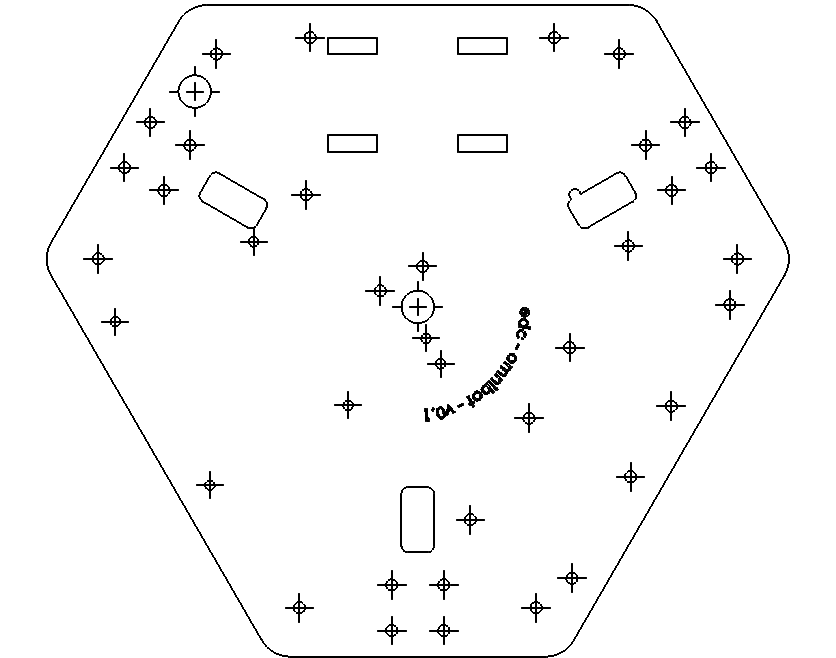
\includegraphics[width = 0.45\textwidth]{imagens/chassidxf}
  \caption{Chassi projetado.}
  \label{fig:chassi}
\end{figure}

Todos os componentes adquiridos possuem furos para fixação por meio de parafusos com 3 mm de diâmetro. A estrutura foi projetada com furos de 3,5 mm de diâmetro, para compensar possíveis erros de medição (visto que nem todos os componentes apresentaram seus desenhos nas informações técnicas) e possíveis tolerâncias de fabricação. Além dos furos de fixação dos componentes, também foram introduzidos orifícios próximos aos motores, para passagem dos cabos de um lado a outro da placa, e orifícios para fixação da bateria com presilhas plásticas. Na mesma área destinada à fixação da bateria, se adicionou furação capaz de receber uma placa Arduino MEGA, caso se deseje utilizar um microcontrolador em trabalhos futuros. Também foram adicionados 6 furos na periferia do chassi, para possibilitar a montagem de outra chapa sobre a dos componentes, caso sejam realizados trabalhos que exijam a expansão da estrutura.

A plataforma projetada foi então fabricada, utilizando chapas de acrílico transparente de 5 mm de espessura. Se cogitou produzir tal estrutura em alumínio, porém optou-se por utilizar o acrílica por conta da facilidade de obtenção, baixo custo, isolamento elétrico (permitindo montar os componentes eletrônicos diretamente sobre o chassi) e a possibilidade de fabricação utilizando uma máquina de corte a \textit{laser}. A espessura foi escolhida empiricamente, dentro das disponíveis, de maneira relativamente conservadora, e atendeu as necessidades. Na Figura \ref{fig:montagem} se pode ver a montagem final do protótipo.

\begin{figure}[h]
  \centering
  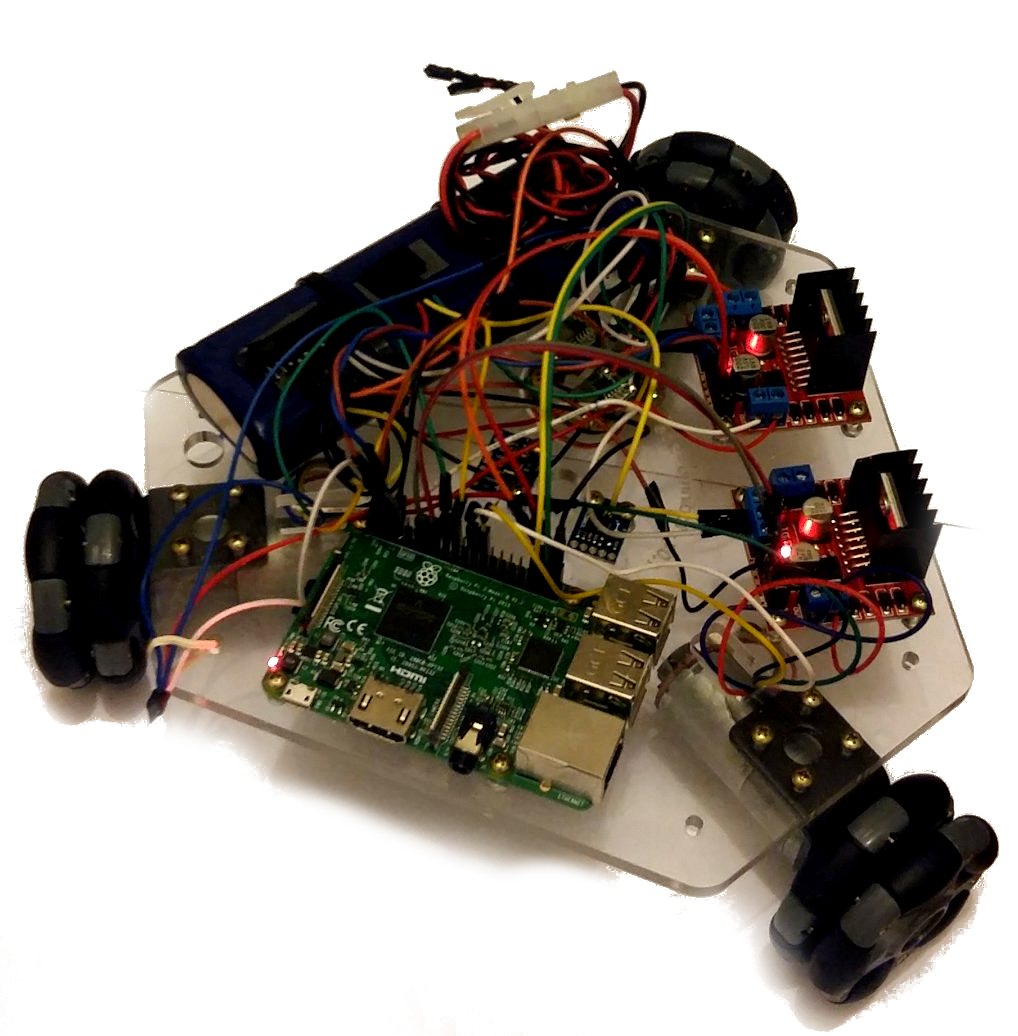
\includegraphics[width = 0.45\textwidth]{imagens/roboto}
  \caption{Protótipo montado, sem as canetas.}
  \label{fig:montagem}
\end{figure}

A bateria foi fixada sobre a estrutura utilizando presilhas plásticas. Ao redor da bateria foram fixados 3 barramentos, para aterramento, alimentação dos \textit{drivers} e alimentação dos \textit{encoders}. Foram instalados um conector para a bateria e outro conector para o caso em que se deseja utilizar uma fonte externa.  Além dos fios que alimentam os reguladores de tensão, um par de fios sobressalente (conectados ao terminal positivo e negativo da fonte ou bateira) foi instalado junto a estes conectores, e pode ser utilizado em trabalhos futuros.

O custo de aquisição dos componentes selecionados pode ser visto detalhado no \hyperref[sec:custo]{Apêndice A}. Cabe ressaltar que todos os itens foram comprados em dobro, para realizar a montagem de dois robôs para futuros trabalhos no LAMECC (Laboratório de Mecatrônia e Controle). Mais detalhes sobre as dimensões do chassi podem ser vistos no diagrama apresentado no \hyperref[sec:draw]{Apêndice C}.

\section{Desenvolvimento Teórico}
\label{sec:teorico}

%% MODELAGEM:
%PARK: pg 468
\subsection{Modelagem Cinemática}

Para o desenvolvimento do trabalho, é necessário obter um modelo matemático para o sistema. Este modelo relaciona o ambiente com o robô e suas partes, em termos de posições e velocidades. Primeiramente, se definem dois sistemas de coordenadas. O primeiro, $(x_I,y_I)$, é o sistema de coordenadas global, fixo no ambiente. O segundo, $(x_R,y_R)$, está centrado no próprio robô. Ainda se pode definir o ângulo $\theta$ como a orientação do robô -- ou seja, o ângulo entre os dois sistemas de coordenadas. Tal relação pode ser vista na Figura \ref{fig:ref}, e a transformação de um sistema para o outro é descrita na Equação \ref{eq:world_ref}, conforme \citet{siegwart2011introduction} e \citet{ritter2016modelagem}.

\begin{figure}[h]
  \centering
  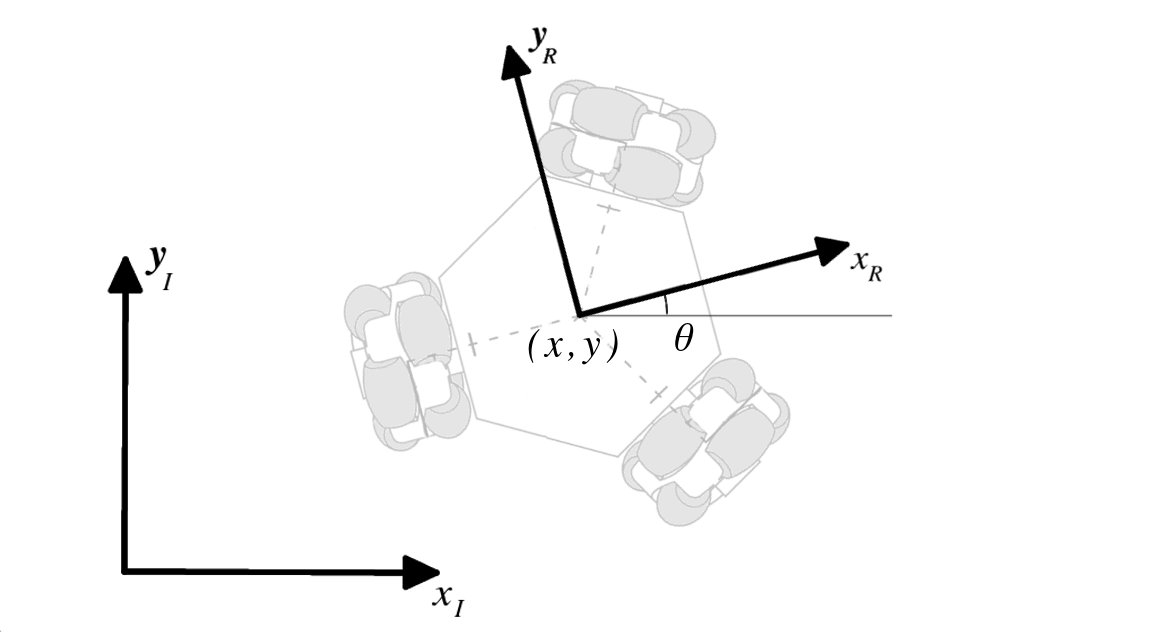
\includegraphics[width = 0.65\textwidth]{imagens/ref}
  \caption{Sistemas de coordenadas global I e relativo ao centro do robô R.}
  \source{Adaptado de \citet{ritter2016modelagem}}
  \label{fig:ref}
\end{figure}

\begin{equation}
  \begin{pmatrix}
    x_I \\
    y_I \\
    \theta
  \end{pmatrix}
  =
  \begin{pmatrix}
    cos \theta & -sen \theta & 0 \\
    sen\theta  &  cos \theta & 0 \\
    0          & 0          & 1
  \end{pmatrix}
  \begin{pmatrix}
    x_R \\
    y_R \\
    \theta
  \end{pmatrix}
  \label{eq:world_ref}
\end{equation}

O último termo da Equação \ref{eq:world_ref} também pode ser descrito como $q_R$, e o vetor de velocidades $[v_x, v_y, \omega_z]^T$, centrados no sistema de coordenadas do robô, é $\dot{q_R}$. Com o objetivo de mapear a velocidade de giro das rodas $\dot{\phi} = [\dot{\phi}_1, \dot{\phi}_2, \dot{\phi}_3]^T$ às velocidades $\dot{q_R}$, se utiliza a modelagem cinemática apresentada por \citet{siegwart2011introduction}, com as referências apresentadas na Figura \ref{fig:robo_vel}. Na figura,  A mesma modelagem é utilizada por \citet{ritter2016modelagem}, porém com outra sequência e sentido de giro para as rodas.

\begin{figure}[h]
  \centering
  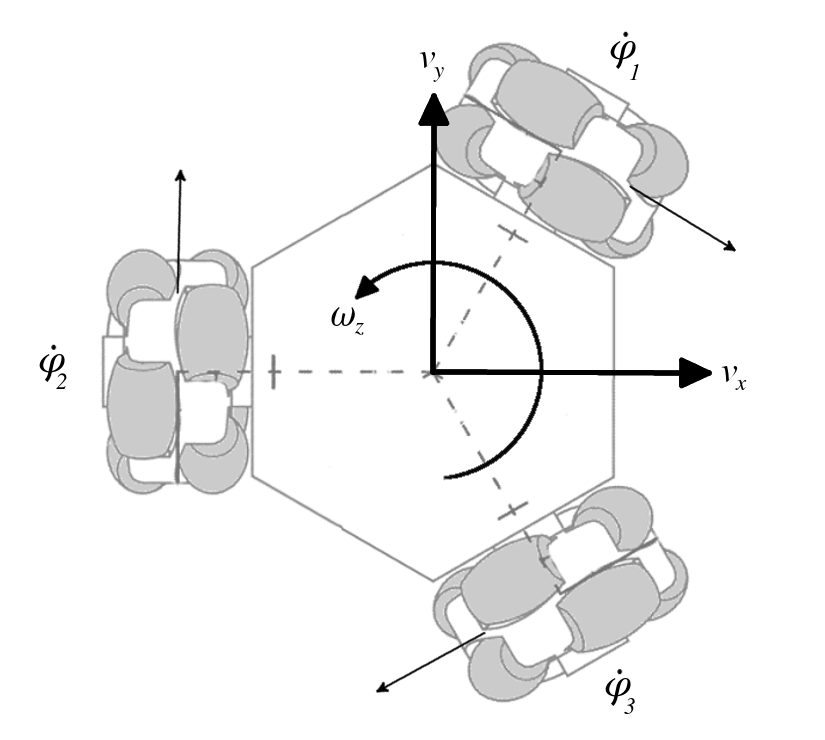
\includegraphics[width = 0.5\textwidth]{imagens/robot_vel4}
  \caption{Vista superior do robô, mostrando as convenções adotadas. As grandezas $v_x$ e $v_y$ estão no sistema de coordenadas do robô.}
  \label{fig:robo_vel}
\end{figure}

Assim, para um robô com 3 rodas dispostas em simetria radial em torno do centro da estrutura, a cinemática direta é dada pela Equação \ref{eq:dk}. Diversos autores utilizam variações da mesma modelagem (\citet{rojas2006holonomic}, \citet{pin1994new}, entre outros). Nas equações apresentadas, $r$ é o raio de cada roda e $R$ o raio do robô (a distância do centro da roda ao centro da estrutura do robô).

\begin{equation}
  \begin{pmatrix}
    v_x \\
    v_y \\
    \omega_z
  \end{pmatrix}
  =
  \frac{r}{3R}
  \begin{pmatrix}
    -\frac{3R}{\sqrt{3}} & 0   & \frac{3R}{\sqrt{3}} \\
    R                    & -2R & R                   \\
    1                    & 1   & 1
  \end{pmatrix}
  \begin{pmatrix}
    \dot{\phi_1} \\
    \dot{\phi_2} \\
    \dot{\phi_3}
  \end{pmatrix}.
  \label{eq:dk}
\end{equation}

Também se deseja utilizar a cinemática inversa do modelo, obtida realizando-se a inversão da matriz de transformação apresentada na Equação \ref{eq:dk}, é dada pela Equação \ref{eq:ik}. Nota-se que esta inversão é simplificada no caso do robô com 3 rodas, visto que quando há mais rodas é formada uma matriz $3 \times n$, sendo $n$ o número de rodas, e se deve utilizar uma matriz pseudo-inversa, conforme demonstrado por \citet{rojas2006holonomic}.

\begin{equation}
  \begin{pmatrix}
    \dot{\phi_1} \\
    \dot{\phi_2} \\
    \dot{\phi_3}
  \end{pmatrix}
  =
  \frac{1}{r}
  \begin{pmatrix}
    -\frac{\sqrt{3}}{2} & \frac{1}{2} & R \\
    0                   & -1          & R \\
    \frac{\sqrt{3}}{2}  & \frac{1}{2} & R
  \end{pmatrix}
  \begin{pmatrix}
    v_x \\
    v_y \\
    \omega_z
  \end{pmatrix}
  \label{eq:ik}
\end{equation}

Como pela classificação de \citet{campion1996structural} um \acrshort{tomr} é caracterizado na categoria (3,0), o modelo cinemático das equações \ref{eq:dk} e \ref{eq:ik} é controlável, estável e descreve a posição, orientação e suas derivadas de forma suficiente. % O modelo cinemático da Equação \ref{eq:dk} também é utilizado por \citet{rojas2006holonomic} e \citet{ritter2016modelagem}.

%% ODOMETRIA:
% lynch, pg 492 do pdf
\subsection{Odometria}

Após movimentações, se torna necessário calcular a nova posição do robô, para que se possa relacionar novamente o robô ao ambiente utilizando as relações obtidas da modelagm. Para o cálculo da odometria, se utiliza a metodologia mostrada em \citet{lynch2017modern}. Se assume que durante um certo intervalo de tempo $\Delta t$ se tenha velocidades de rotação constantes nas rodas, o que permite considerar $\dot{\phi_i}.\Delta t = \Delta \phi_i$. Considera-se também que a unidade de tempo deste período é arbitrária, e como se deseja integrar no mesmo intervalo posteriormente, se assume um período unitário $\Delta t = 1$. Este procedimento está descrito na Equação \ref{eq:odo}, modificada a partir da Equação \ref{eq:dk}. Na prática, é fácil contar os deslocamentos angulares $\Delta \phi_i$, visto que o número de pulsos por revolução dos \textit{encoders} é determinado.

\begin{equation}
  \begin{pmatrix}
    v_x \\
    v_y \\
    \omega_z
  \end{pmatrix}
  =
  \frac{r}{3R}
  \begin{pmatrix}
    -\frac{3R}{\sqrt{3}} & 0   & \frac{3R}{\sqrt{3}} \\
    R                    & -2R & R                   \\
    1                    & 1   & 1
  \end{pmatrix}
  \begin{pmatrix}
    \Delta{\phi_1} \\
    \Delta{\phi_2} \\
    \Delta{\phi_3}
  \end{pmatrix}.
  \label{eq:odo}
\end{equation}

De posse das velocidades da plataforma durante o período de tempo unitário $\Delta t$ -- lembrando que $v_x$, $v_y$ e $\omega_z$ estão no sistema de coordenadas centrado no corpo do robô --, se deve avaliar o deslocamento em relação ao centro do robô na posição anterior. Para o caso em que $\omega_z = 0$, numa trajetória retilínea, se tem simplesmente que $\Delta q_R = \dot{q_R}$.

No entanto, quando houve mudança de orientação no período e consequentemente $\omega_z \neq 0$, se deve levar em consideração os desvios de trajetória causados por essa rotação. Assim, se obtem $\Delta q_R$ de acordo com a Equação \ref{eq:desvio} \citep{lynch2017modern}.

\begin{equation}
  \Delta q_R
  =
  \begin{pmatrix}
    \Delta x_R \\
    \Delta y_R \\
    \Delta\theta
  \end{pmatrix}
  =
  \begin{pmatrix}
    (v_x sen(\omega_z)) + v_y (cos(\omega_z) - 1)/\omega_z \\
    (v_y sen(\omega_z)) + v_x (1-cos(\omega_z)) / \omega_z \\
    \omega_z
  \end{pmatrix}
  \label{eq:desvio}
\end{equation}

Sendo $k$ o instante antes do período de tempo analisado, para se obter a nova posição $q_I$ do robô no sistema de coordenadas global se deve utilizar a rotação $R(\theta_k)$ apresentada na Equação \ref{eq:world_ref}, e atualizando os valores da última iteração conforme a Equação \ref{eq:new_odo}.

\begin{equation}
  q_{I(k+1)} = q_{I(k)} + \Delta q_I = q_{I(k)} + R(\theta_k) \Delta q_I
  \label{eq:new_odo}
\end{equation}
%\cite{samani2007comprehensive}: Adicionam um modelo de ruído dos encoders à estimativa. TIRAR OU ELABORAR?

%% PLANEJAMENTO DE TRAJETÓRIA:
\subsection{Planejamento de Trajetória}

Para o robô desenvolvido, não há a necessidade de implementar algoritmos complexos de planejamento de trajetória (detecção de obstáculos, caminhos de mínima energia, etc.). Serão abordados caminhos ``ponto a ponto'', que levam de um ponto inicial a um ponto final, ambos em repouso \citep{lynch2017modern}.

Apesar de ser uma trajetória simples, ainda se podem aplicar considerações para uma melhor operação do sistema. Uma dessas considerações é o chamado \textit{time-scaling} da trajetóra, ou seja, a geração de uma função $s(t)$ que suavize o comportamento do robô por meio de restrições em velocidades e acelerações. Na Figura \ref{fig:poly5} se pode ver uma curva de perfil de velocidade polinomial de quinta ordem, que pode garantir velocidades e acelerações nulas nos pontos de origem e destino.

\begin{figure}[h]
  \centering
  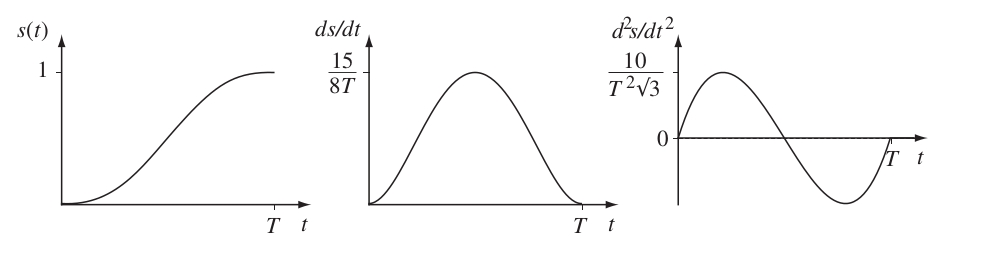
\includegraphics[width = 0.85\textwidth]{imagens/poly5}
  \caption{Deslocamento, velocidade e aceleração durante uma trajetória gerada por polinômio de quinta ordem. Aceleração e velocidade são nulas tanto no ponto de origem quanto no ponto de destino.}
  \source{\citet{lynch2017modern}}
  \label{fig:poly5}
\end{figure}

No entanto, a interpolação de um polinômio a cada cálculo de trajetória é um processo que pode envolver um certo custo computacional elevado, e devido à simplicidade dos componentes utilizados, se julgou que o aumento de suavidade na operação não fosse significativo. Portanto, neste trabalho se optou por utilizar um perfil de velocidade trapezoidal, conforme mostrado na Figura \ref{fig:trap}. Tal perfil é um dos mais comuns em robótica, devido a sua simples implementação. Os limites de aceleração foram definidos na fase de implantação do \textit{software}, de modo a evitar o deslizamento das rodas utilizadas na superfície de testes.

\begin{figure}[h]
  \centering
  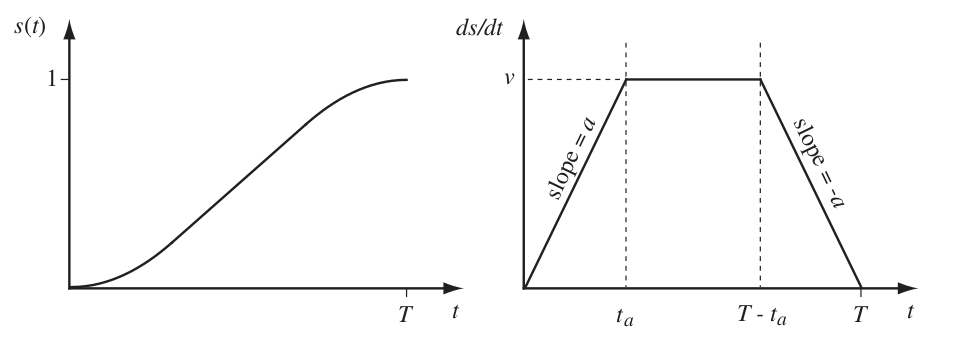
\includegraphics[width = 0.63\textwidth]{imagens/trapezoidal}
  \caption{Deslocamento e velocidade durante um deslocamento com perfil de velocidades trapezoidal. Tal perfil foi adotado neste trabalho.}
  \source{\citet{lynch2017modern}}
  \label{fig:trap}
\end{figure}

Utilizando a curva do perfil de velocidade, se pode fixar setpoints de velocidade para cada ponto.

%% CONTROLE:
\subsection{Controle}

A teoria de controle aplicada a robos móveis é bastante ampla, sendo utilizadas na prática diversas técnicas. O controle do tipo PID, no entanto, ainda é um dos mais utilizados, pela sua simplicidade de implementação e resultados bastante eficazes. O controle utilizado no robô de certa maneira acompanha a modelagem desenvolvida: trabalhos que envolvem modelagens dinâmicas utilizam controladores PID que levam os aspectos dinâmicos em consideração \citep{samani2007comprehensive}, enquanto que o mesmo tipo de controlador pode também ser utilizado quando o modelo disponível, como neste trabalho, é cinemático \citep{indiveri2009swedish}.

Para implementar o controle de velocidade do robô, se tem duas opções para o conjunto de variáveis controladas. Se pode controlar as velocidades do corpo do robô, $v_x$, $v_y$ e $\omega_z$, sendo a saída de cada controlador sobreposta para acionamento das rodas, como feito por \citet{rojas2006holonomic}, que se beneficiam deste esquema pois seu robô foi construído com 4 rodas, o que tornaria necessário um controlador a mais. A outra maneira é controlando a velocidade de cada motor independentemente, a partir dos dados recebidos dos cálculos de cinemática. Tal abordagem foi utilizada no presente trabalho, devido ao modo como havia sida implementada a cinemática por \cite{ritter2016modelagem} -- a ser discutido mais adiante. Se pode ver um esquema do sistema utilzado na Figura \ref{fig:controle}.

\begin{figure}[h]
  \centering
  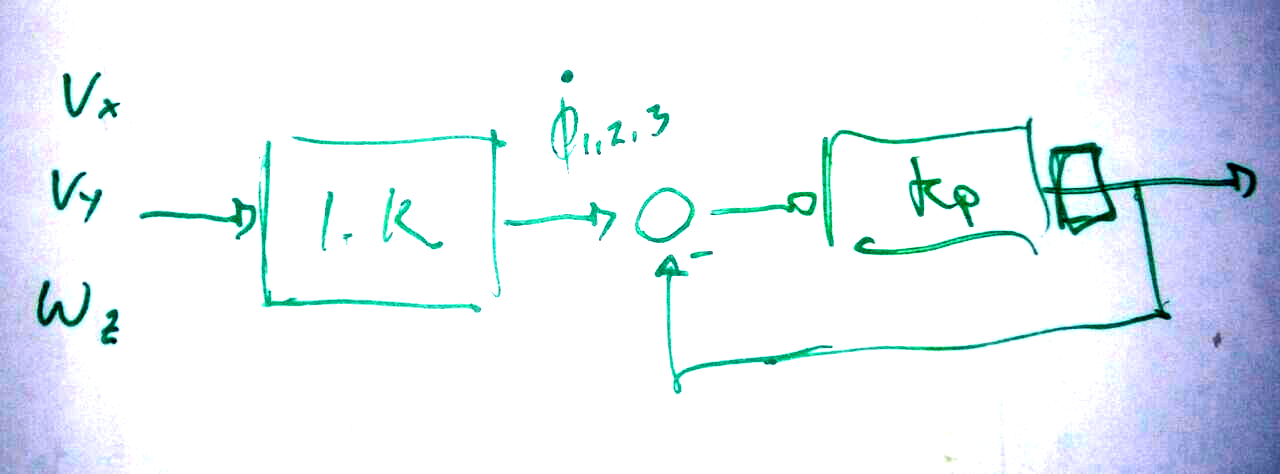
\includegraphics[width = 0.75\textwidth]{imagens/controle}
  \caption{Arquitetura de controle utilizada.}
  %\source{\citet{lynch2017modern}}
  \label{fig:controle}
\end{figure}

O sistema de controle foi implementado em um programa de computador, e portanto não é contínuo. Num sistema digital, a atualização dos valores ocorre apenas uma vez a cada período de tempo $T$, conforme a Equação \ref{eq:pidorf}. Sendo $K_P$, $K_I$ e $K_D$ os termos que multiplicam, respectivamente, o erro, a integral do erro e a taxa de variação do erro no caso de um sistema de controle contínuo, $u$ o sinal de controle e $x$ a grandeza controlada. \citep{dorf2008modern}

\begin{equation}
  u[k] = (K_P+K_I T+\frac{K_D}{T})\ x[k] - K_D T\ x[k-1] + K_I\ u[k-1]
  \label{eq:pidorf}
\end{equation}

Em um sistema como um motor elétrico, ganhos mais altos costumam tornar a resposta do sistema mais rápida. Em uma aplicação real, entretanto, ganhos grandes acarretam em saturação de atuadores, mudanças repentinas de torque, vibrações na estrutura e até mesmo instabilidade. \citep{lynch2017modern}

Outro fator inerente das aplicações de sistemas de controle é a possível presença de não-linearidades. Em motores elétricos que utilizam um trem de engrenagens como redução mecânica é muito comum haver a não-linearidade chamada de ``zona-morta'', conforme mostrado na Figura \ref{fig:zonamorta}. Como se pode ver no gráfico da esquerda, um atuador só responde para valores do sinal de controle $u_{eq}$ acima de $z_{md}$ ou abaixo de $z_{me}$. A compensação é simples, como se pode ver no gráfico da direita: se adiciona ao sinal de controle calculado $u_{ec}$ um coeficiente, no caso de sinal positivo. No caso de sinal negativo, se subtrai um coeficiente. Nota-se que nem sempre a zona morta é simétrica.

\begin{figure}[h]
  \centering
  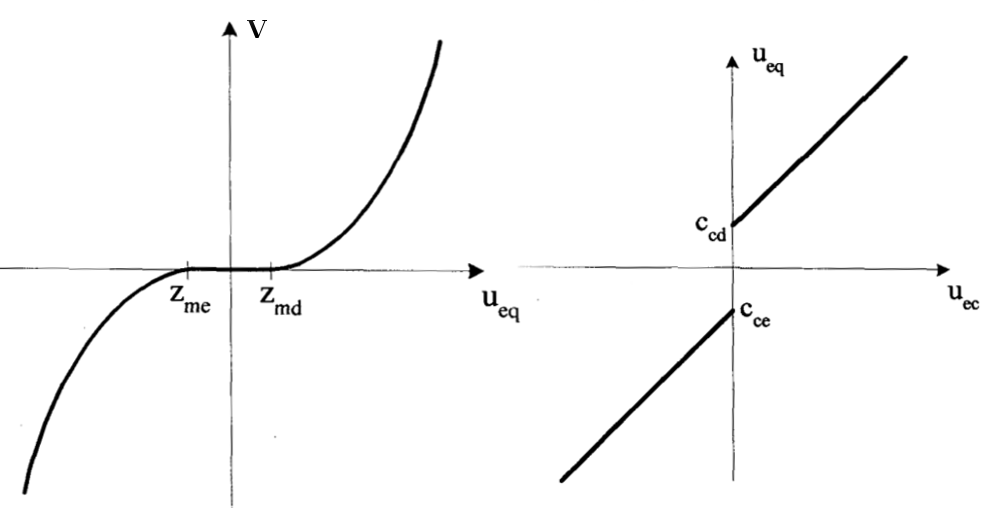
\includegraphics[width = 0.65\textwidth]{imagens/zonamorta0}
  \caption{Zona morta em um atuador e um tipo de correção a ser aplicada no sinal de controle.}
  \source{Adaptado de \citet{cunha2001zm}}
  \label{fig:cont_zm}
\end{figure}

O controle de posição de um robô móvel, de acordo com \citet{siegwart2011introduction}, pode ser de três tipos. Se pode desejar atingir uma certa configuração estática, seguir uma trajetória dependentente do tempo ou seguir um caminho geométrico. As soluções mais precisas utilizam controle com realimentação, e dependem fortemente do bom funcionamento do sistema de odometria \citep{samani2007comprehensive}. Há, também, robôs que operam em malha aberta, decompondo trajetórias em trajetos simples (retas e curvas). Nessa estratégia, o controle se torna um problema de computar com antecedência ao movimento o perfil de velocidade a ser executado \citep{siegwart2011introduction}.

\subsection{Limitações de Velocidade}

É importante ressaltar que toda a cinemática desenvolvida nas subseções anteriores não considera limites de velocidade para os atuadores. Numa aplicação real, entretanto, existe um ponto de saturação no acionamento de cada motor, que deve ser levada em consideração. Na Figura \ref{fig:twist_sat} se pode ver o efeito dessas limitações, conforme descrito em \citet{lynch2017modern}.

\begin{figure}[h]
  \centering
  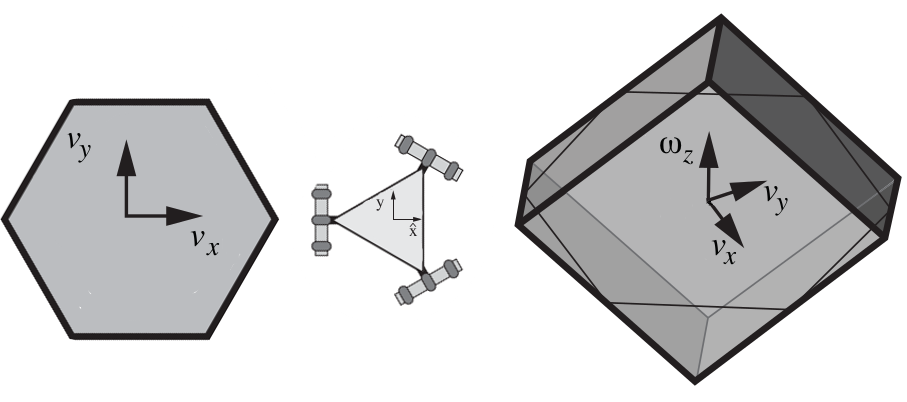
\includegraphics[width = 0.63\textwidth]{imagens/twist_sat}
  \caption{Limites de velocidade translacional e rotacional em função dos limites de saturação dos motores reais.}
  \source{Adaptado de \citet{lynch2017modern} para as coordenadas utilizadas.}
  \label{fig:twist_sat}
\end{figure}

Quando não há rotações ($\omega_z = 0$), o limite de velocidade do corpo do robô é descrito pelo hexágono mostrado na porção esquerda da Figura \ref{fig:twist_sat}: a maior velocidade possível é na direção em que uma das rodas está sendo ``arrastada'', e as componentes de velocidade das outras rodas se somam. Numa situação em que haja necessidade de rotação, a velocidade angular do robô se torna limitada da maneira mostrada no volume tridimensional à direita da Figura \ref{fig:twist_sat}, e se torna fácil enxergar que, para realizar um movimento de rotação na maior velocidade ângular possível, não se pode ter movimentos de translação, para que todos os componentes de velocidade das rodas contribuam apenas para a rotação.

Se pode dizer, então, que para aplicações reais nas quais a holonomicidade da plataforma é de fato desejável, se deve implantar um sistema de planejamento de trajetória que leve em consideração as limitações de velocidade descritas acima.

\section{Implementação dos algoritmos}
\label{sec:software}

Os aspectos teóricos desenvolvidos na seção anterior foram implementados em software para a aplicação prática do sistema. Na Figura \ref{fig:sistema} se pode enxergar o sistema proposto inicialmente. Foram omitidos da figura, por simplicidade, os algoritmos de limitação de velocidade, compensação de zona-morta e geração de trajetórias.

\begin{figure}[h]
  \centering
  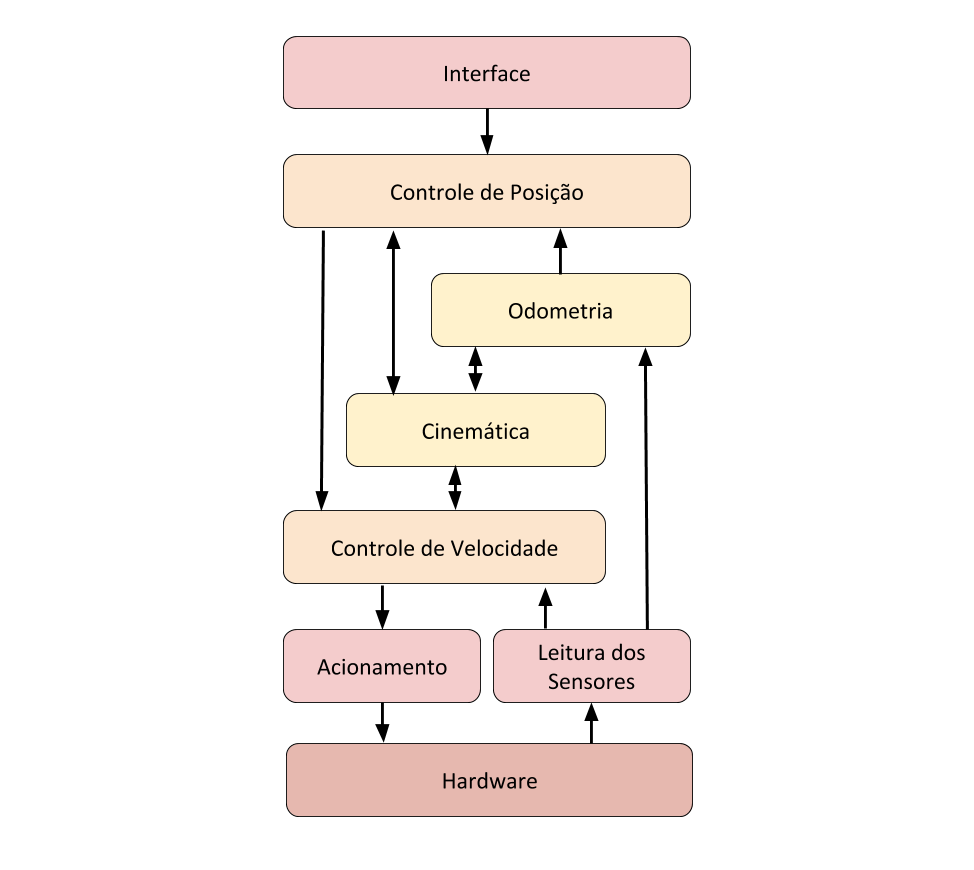
\includegraphics[width = 0.6\textwidth]{imagens/sistema}
  \caption{Estrutura e hierarquia dos subsistemas propostos inicialmente.}
  \label{fig:sistema}
\end{figure}

O \textit{software} foi implementado em um computador embarcado Raspberry Pi, conforme proposto por \citet{ritter2016modelagem}, utilizando a linguagem C++, uma das linguagens suportadas pelas bibliotecas de acesso às portas \acrshort{gpio} que apresenta melhores velocidades de execução. Com esta escolha de linguagem, também se pode utilizar parcialmente os códigos implementados para o trabalho de \citet{ritter2016modelagem}, também escritos em C++.

%Uma preocupação que se tem ao utilizar um computador se deve ao fato do mesmo não ser caracterizado como um sistema de tempo real. No caso, temporização precisa não é garantida, e a ordem de prioridade de execução de tarefas é gerenciada pelo \textit{kernel VERIFICA}. Assim, funções que seriam executadas imediatamente em um microcontrolador (como rotinas de interrupção), são executadas ``assim que possível'', o que pode prejudicar o desempenho do sistema.


%ordem das coisas:
%-análise dos códigos de cinemática
%-desmembramento das funções do ritter

A primeira etapa do desenvolvimento foi a de separar o código desenvolvido por \citet{ritter2016modelagem} em duas partes: uma destinada aos comandos de acionamento, que naquele trabalho eram realizados em um simulador, e outra relacionada à modelagem cinemática do robô. Esta segunda porção foi encapsulada em uma biblioteca, analisada e testada no computador embarcado.

%-código de acionamento dos motores
%-bilbioteca orientada a objetos para o acionamento de cada motor e modularização do código\\
Em seguida, foram realizados testes de acionamento e leitura dos sensores dos motores, a biblioteca PIGPIO \citep{pigpio} para a utilização das entradas e saídas físicas do computador. Utilizando o conceito de orientação a objetos, foi criada uma classe que descreve os parâmetros de cada conjunto motor/sensor e as operações a serem realizadas sobre eles. Esta classe foi batizada de ``RPiInterface'', pois realiza a interface entre o processamento da Raspberry Pi com os sensores e atuadores físicos.
%-controle de velocidade
Na mesma classe se implementou a função de atualização da lei de controle de velocidade de cada motor, com variáveis destinadas aos ganhos proporcional, integral e derivativo pré-alocadas.

Para os testes iniciais, foi inicializado apenas o ganho proporcional, e a lei de controle similiar a da Equação \ref{eq:pidorf} foi aplicada nos três motores, sendo executada a cada 10 ms. Este período arbitrário foi escolhido por ser o menor permitido por uma das funções da biblioteca Pigpio, mas de fácil substituição. No entanto, este controlador apresentou bons resultados durante os testes, e a única mudança realizada durante o desenvolvimento do trabalho foram alguns ajustes do ganho $K_P$.

Após esta configuração inicial do controlador, foram revisadas as constantes dimensionais em \cite{ritter2016modelagem}. O encoder é dividido em 341,2 pulsos por rotação, e a unidade de tempo utilizada para a leitura é de $\mu$s. A biblioteca de cinemática utiliza as velocidades lineares das rodas, em m/s, e utilizando as dimensões do robô, das rodas e as características dos sensores, se encontrou o fator de conversão de uma relação para a outra. Assim, internamente ao programa se têm todas as velocidades na mesma unidade (com exceção da velocidade angular do chassi).

A decodificação dos \textit{encoders} é feito por meio de ``interrupções'' \textit{descobrir como eu posso chamar isso no Linux, Walter não vai gostar.}

%algoritmo de limitação de velocidade, escalonamento \\
Conforme descrito na seção anterior, robôs holonômicos possuem uma limitação de velocidade. Durante a movimentação, caso seja exigida uma velocidade muito alta, pode ocorrer a saturação de algum dos motores. Caso a velocidade desejada continue aumentando, as rodas mais lentas continuarão acelerando enquanto a roda saturada se mantém na mesma velocidade. Este novo conjunto de velocidades para as rodas corresponde a uma trajetória não desejada. Tal efeito pode ser visualizado na Figura \ref{fig:scaling_off}.

\begin{figure}[h]
  \centering
  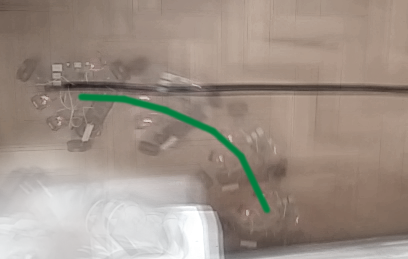
\includegraphics[width = 0.6\textwidth]{imagens/scaling_off}
  \caption{Um motor em saturação, enquanto o robô sofre alteração de trajetória. O caminho preto é a rota desejada.}
  \label{fig:scaling_off}
\end{figure}

Foi implementado um algoritmo similar ao descrito por \citet{indiveri2009swedish}: caso a cinemática resolva para alguma roda uma velocidade acima de um certo limite, esta roda tem sua velocidade fixada no valor máximo, enquanto as outras são diminuídas também, sem perder a proporcionalidade. Na Figura \ref{fig:scaling_on} é mostrado o efeito deste algoritmo na movimentação retílinea do robô (com o mesmo comando da situação anterior). Após experimentos, se fixou este valor limite em 0,45 m/s.

\begin{figure}[h]
  \centering
  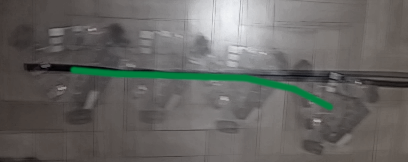
\includegraphics[width = 0.6\textwidth]{imagens/scaling_on}
  \caption{Escalonamento de velocidade ativado.}
  \label{fig:scaling_on}
\end{figure}

%implementação dos algoritmos de odometria
Após a verificação do sistema de controle de velocidade, foram implementadas da maneira descrita na seção anterior a Equação \ref{eq:odo} relacionada à odometria. Para evitar acúmulos de possíveis erros de medição, se evitou utilizar a velocidade computada. Os dados utilizados foram a própria contagem de pulsos de cada \textit{encoder}, e avaliando a taxa de variação desta contagem e de uma contagem imediatamente anterior, se estimaram as velocidades no referencial do robô.

A função de odometria, em tese, é invocada logo antes da lei de controle dos motores ser atualizada, também a cada 10 ms. No entanto, a função não apresentou bons resultados, e deixou de ser utilizada durante os últimos testes. O controle de posição proposto no diagrama da Figura \ref{fig:sistema} teve de ser abandonado, visto que seu desempenho depende da precisão do algoritmo de odometria.

\section{Avaliação experimental}
\label{sec:experimental}

Para validar o desenvolvimento exposto acima, se optou por utilizar um planejamento de trajetória em malha aberta. Foram implementados os modos de movimentação citados por \citet{loh2003mechatronics}: translação retilínea (sem alteração na orientação), rotação pura e uma trajetória híbrida, de translação e rotação. Para cada trajetória foi criada uma função específica, responsável pela geração da trajetória e dos perfis de velocidade a serem seguidos.

No movimento de giro, ilustrado na Figura \ref{fig:giro}, se deseja avaliar a calibração da cinemática, com todas rodas girando ao mesmo tempo (e portanto diminuindo o efeito da zona morta dos motores).

\begin{figure}[h]
  \centering
  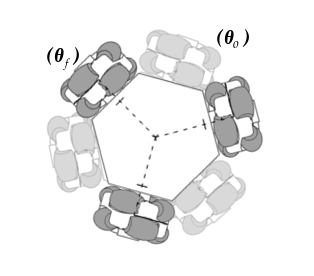
\includegraphics[width = 0.35\textwidth]{imagens/giro}
  \caption{Trajetória de giro.}
  \label{fig:giro}
\end{figure}

Na trajetória retilínea pura, se deseja validar a cinemática desenvolvida, e comprovar a eficiente compensação das não-linearidades dos atuadores e do algoritmo de limitação de velocidade. É a trajetória mostrada na Figura \ref{fig:reta}.

\begin{figure}[h]
  \centering
  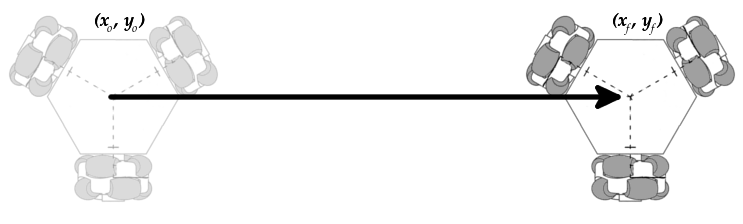
\includegraphics[width = 0.8\textwidth]{imagens/reta}
  \caption{Trajetória retilínea pura.}
  \label{fig:reta}
\end{figure}

Combinando ambas trajetórias, se deseja mover o robô da maneira mostrada na Figura \ref{fig:hibrida}. Para esta trajetória, é necessário recalcular as velocidades de acionamento a cada período de tempo, visto que o sistema referencial do robô é reorientado a cada instante pela rotação do chassi.

\begin{figure}[h]
  \centering
  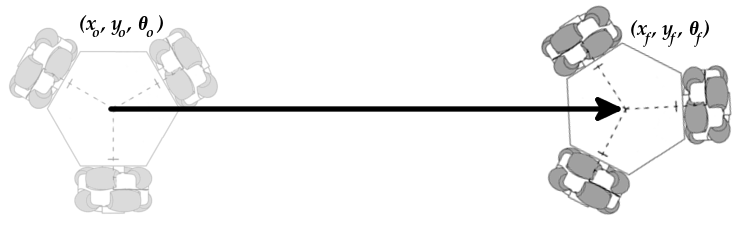
\includegraphics[width = 0.8\textwidth]{imagens/hibrida}
  \caption{Trajetória combinada.}
  \label{fig:hibrida}
\end{figure}

Falar mais algo do experimento?
